\chapter{Modelling Evolution of Life-history Traits}

\section{Modelling Adult Stage}
After modelling larval stage and calibrating, I developed the model for the adult stage of \textit{Drosophila} life cycle. This includes randomly choosing surviving adults from all replicate larval stage vials, matings, and inheritance of larval trait parameters from parents to offspring. Female is mated once with random male chosen from the adult population with replacement for simplicity. From all the offspring produced, eggs are chosen at random with numbers respective to the crowding environment maintained for the next generation.
\subsection{Fecundity}
After each mating, the number of eggs produced for a female are derived from the fecundity equation based on the model of (ref) Tung S. (year). Fecundity is taken as a function of body size of the female and adult nutrition parameter (the amount of yeast provided). Fecundity of an $i^{th}$ female is given as:
\[Egg_{i} = Nut \cdot x_{2} \cdot \log{(x_{3} \cdot s_{i})}\]
Here, $s_{i}$ = body size of the $i^{th}$ female \\
$Egg_{i}$ = Number of eggs laid by the female in a mating \\
$Nut$ = Adult nutrition i.e. the amount of yeast provided \\
$x_{2}, x_{3}$ = scaling parameters
\subsection{Inheritance}
Larval trait parameters (initial feeding rate, effieciency, waste tolerance and critical size) are inherited from parents to offspring produced by each female using mid-parent value. The mid-parent value i.e. average of mother and father for each larval parameter of offspring as mean is calculated for offspring. This mid-parent value is taken as mean of a normal distribution with fixed standard deviation. The standard deviation in this normal distribution determines the heritibility of the mid-parent value and it is considered to be different for each trait parameter. Trait parameters of the offspring are assigned as:
\[T_{i} \in N(mpv_{T}, \delta_{T})\]
Here, \\
$T_{i}$ = Trait parameter assigned to $i^{th}$ offspring from a mating \\
$mpv_{T}$ = Mid-parent value of of the trait $T$ for a given mating \\
$\delta_{T}$ = Stochasticity in mid-parent value of the trait $T$ \\
$N(mpv, \delta)$ = Normal distribution with $mpv$ as mean and $\delta$ as standard deviation
\section{Effect of Laral Crowding on the Evolution of Life-history Traits}
Using initial values for all parameters given in table (no.), the entire model is simulated for 100 generations with 10 replicates for MB, MCU and CCU cultures. All larval trait parameters are taken from independent distribution and there is no correlation between them. To see how larval trait parameters evolve over time, timeseries for these traits of surviving adult individuals are plotted with 95$\%$ CI. \\\\
Initial feeding rate in high density cultures increase over generations at similar rate but inital feeding rate is higher always in CCU culture always than in MCU culture. In MB culture, being control population, initial feeding rate does not evolve (fig ~\ref{fr}).\\\\
Efficiency show similar trend in high density cultures i.e. it increases over generations at similar rate but is higher always in CCU culture always than in MCU culture. In MB culture, being control population, efficiency does not evolve (fig ~\ref{eff}).
\newpage
\begin{figure}
  \centering
  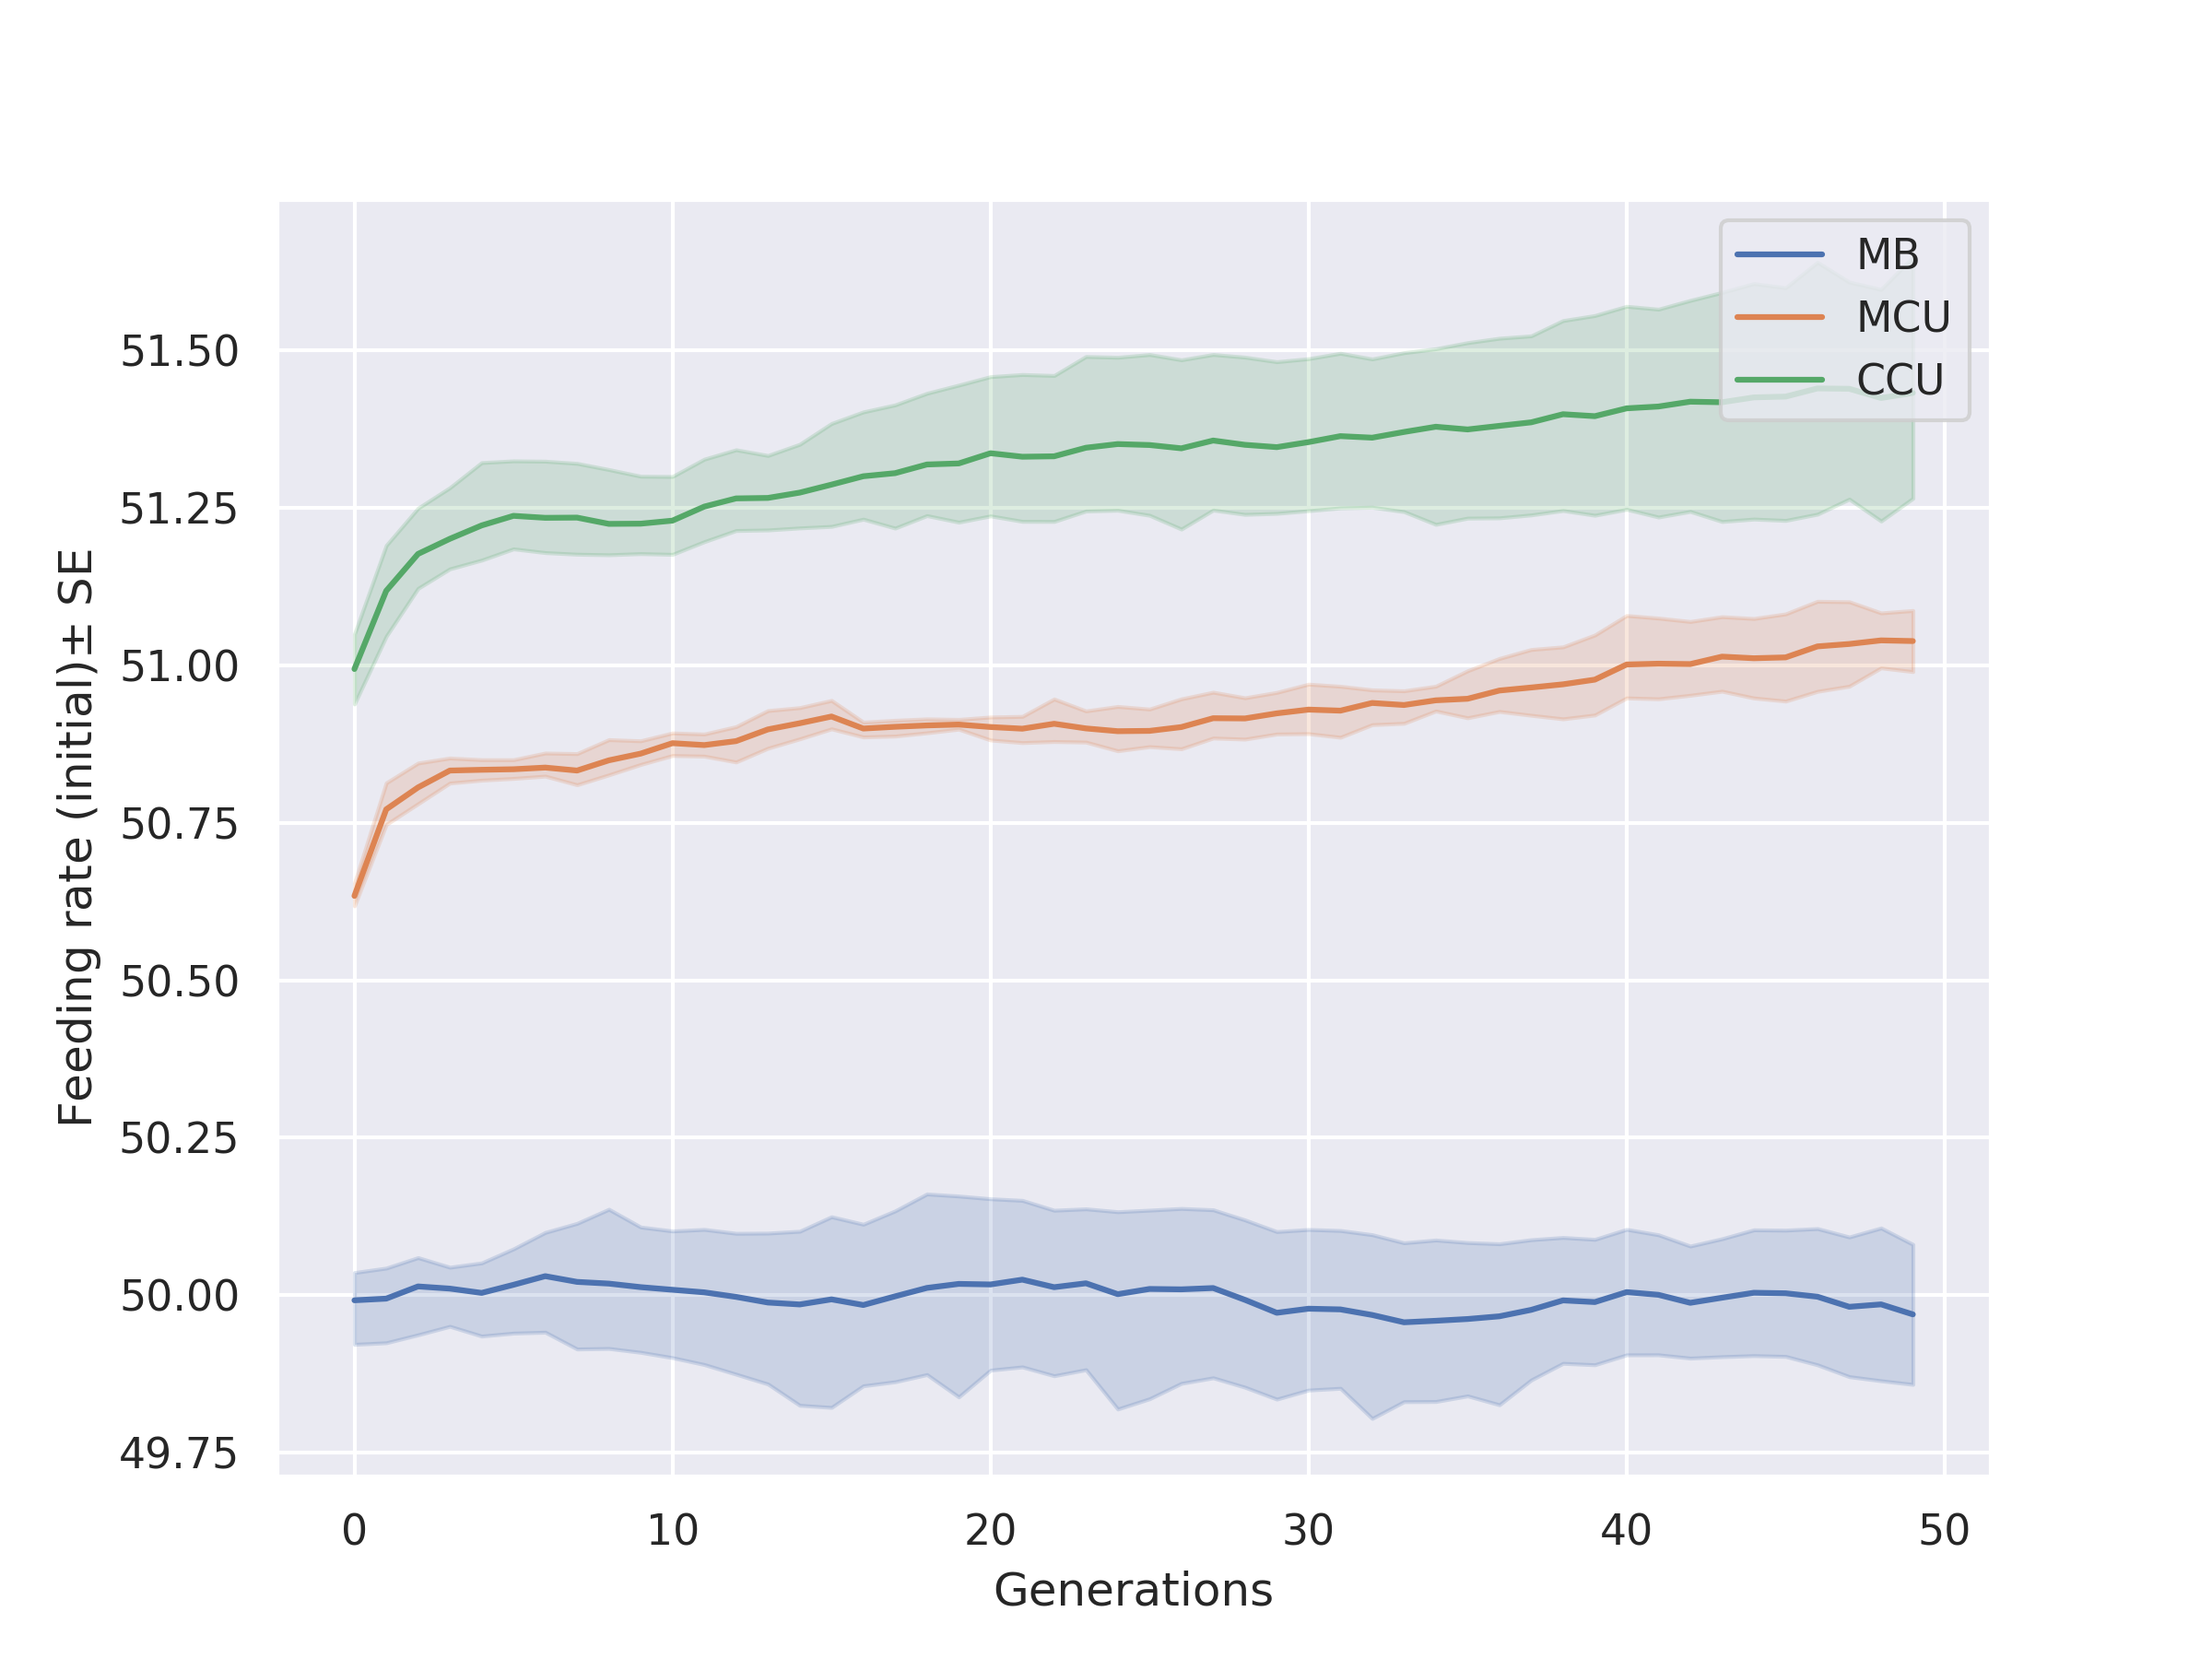
\includegraphics[width=0.9\textwidth]{C4/Figs/fr}
  \caption{Timeseries for initial feeding rate}
  \label{fr}
  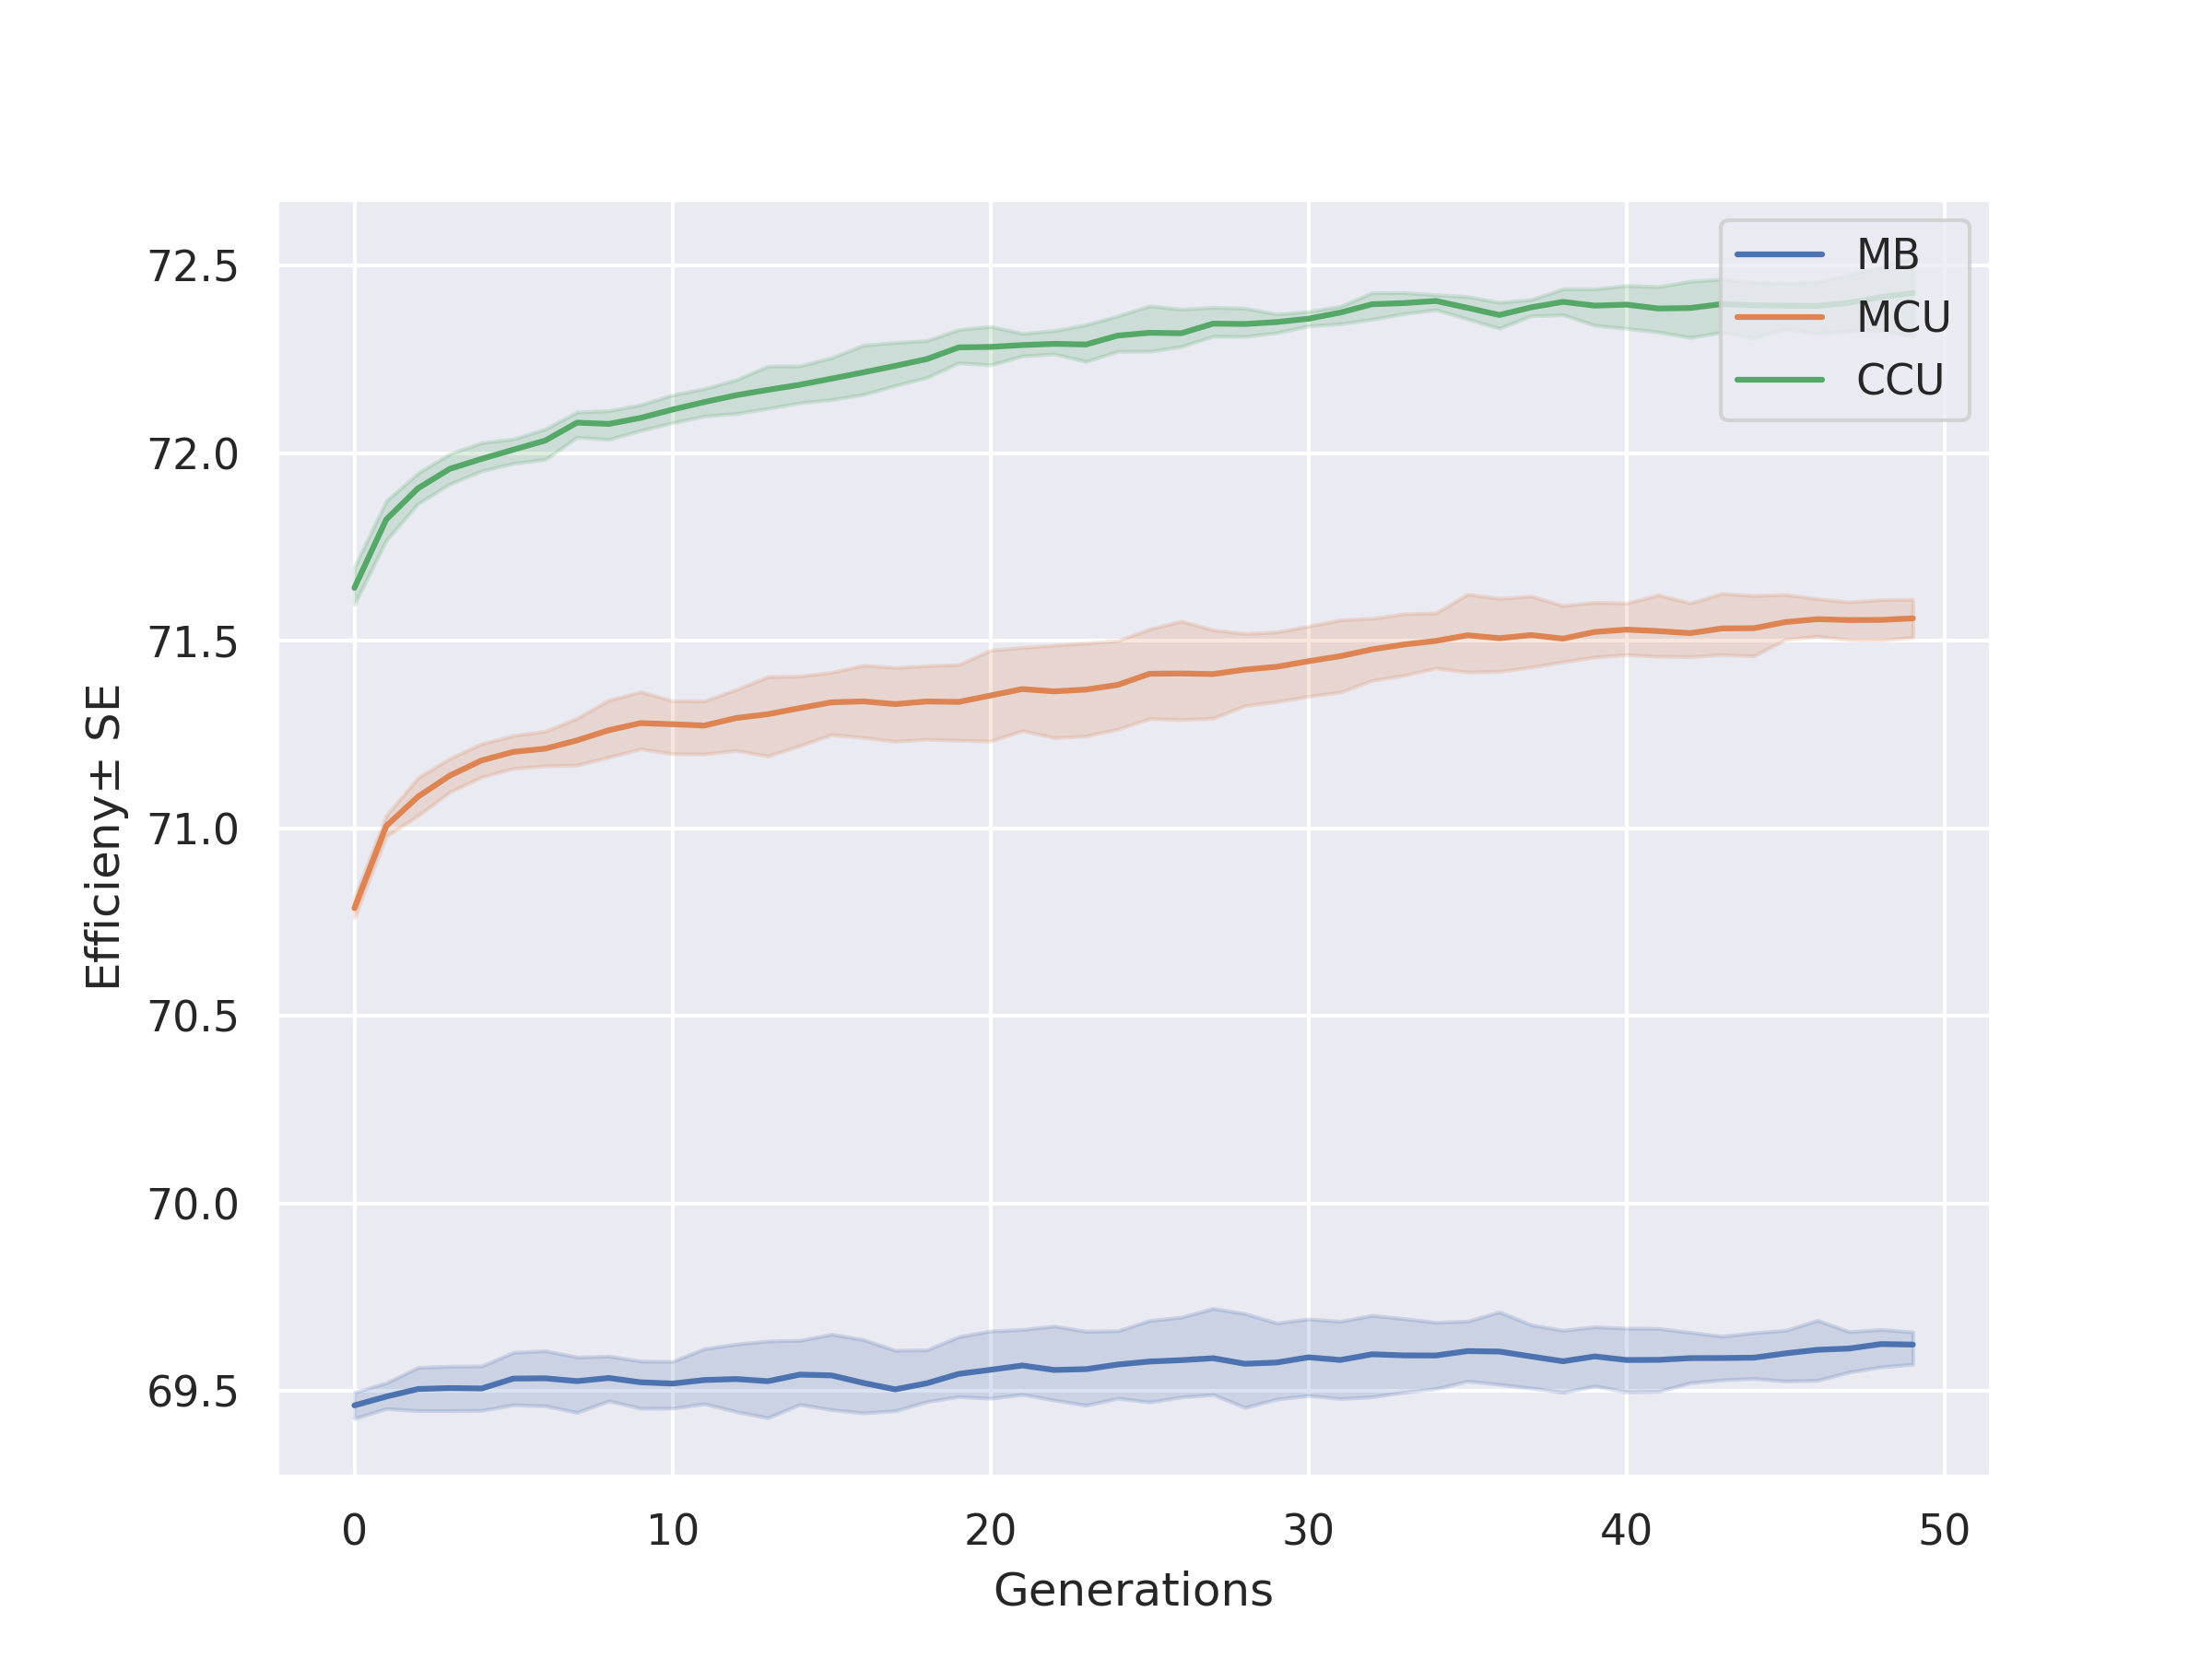
\includegraphics[width=0.9\textwidth]{C4/Figs/eff}
  \caption{Timeseries for initial efficiency}
  \label{eff}
\end{figure}
\newpage
Critical size in high density cultures decreases at the same rate but critical size in CCU culture is always lower than in MCU culture. In MB culture, critical size does not change over generations (fig ~\ref{mc}). \\\\
Waste tolerance does not evolve in all of the culture populations since there is no significant decrease/increase in waste tolerance value (fig ~\ref{wtol}).
\newpage
\begin{figure}[h]
  \centering
  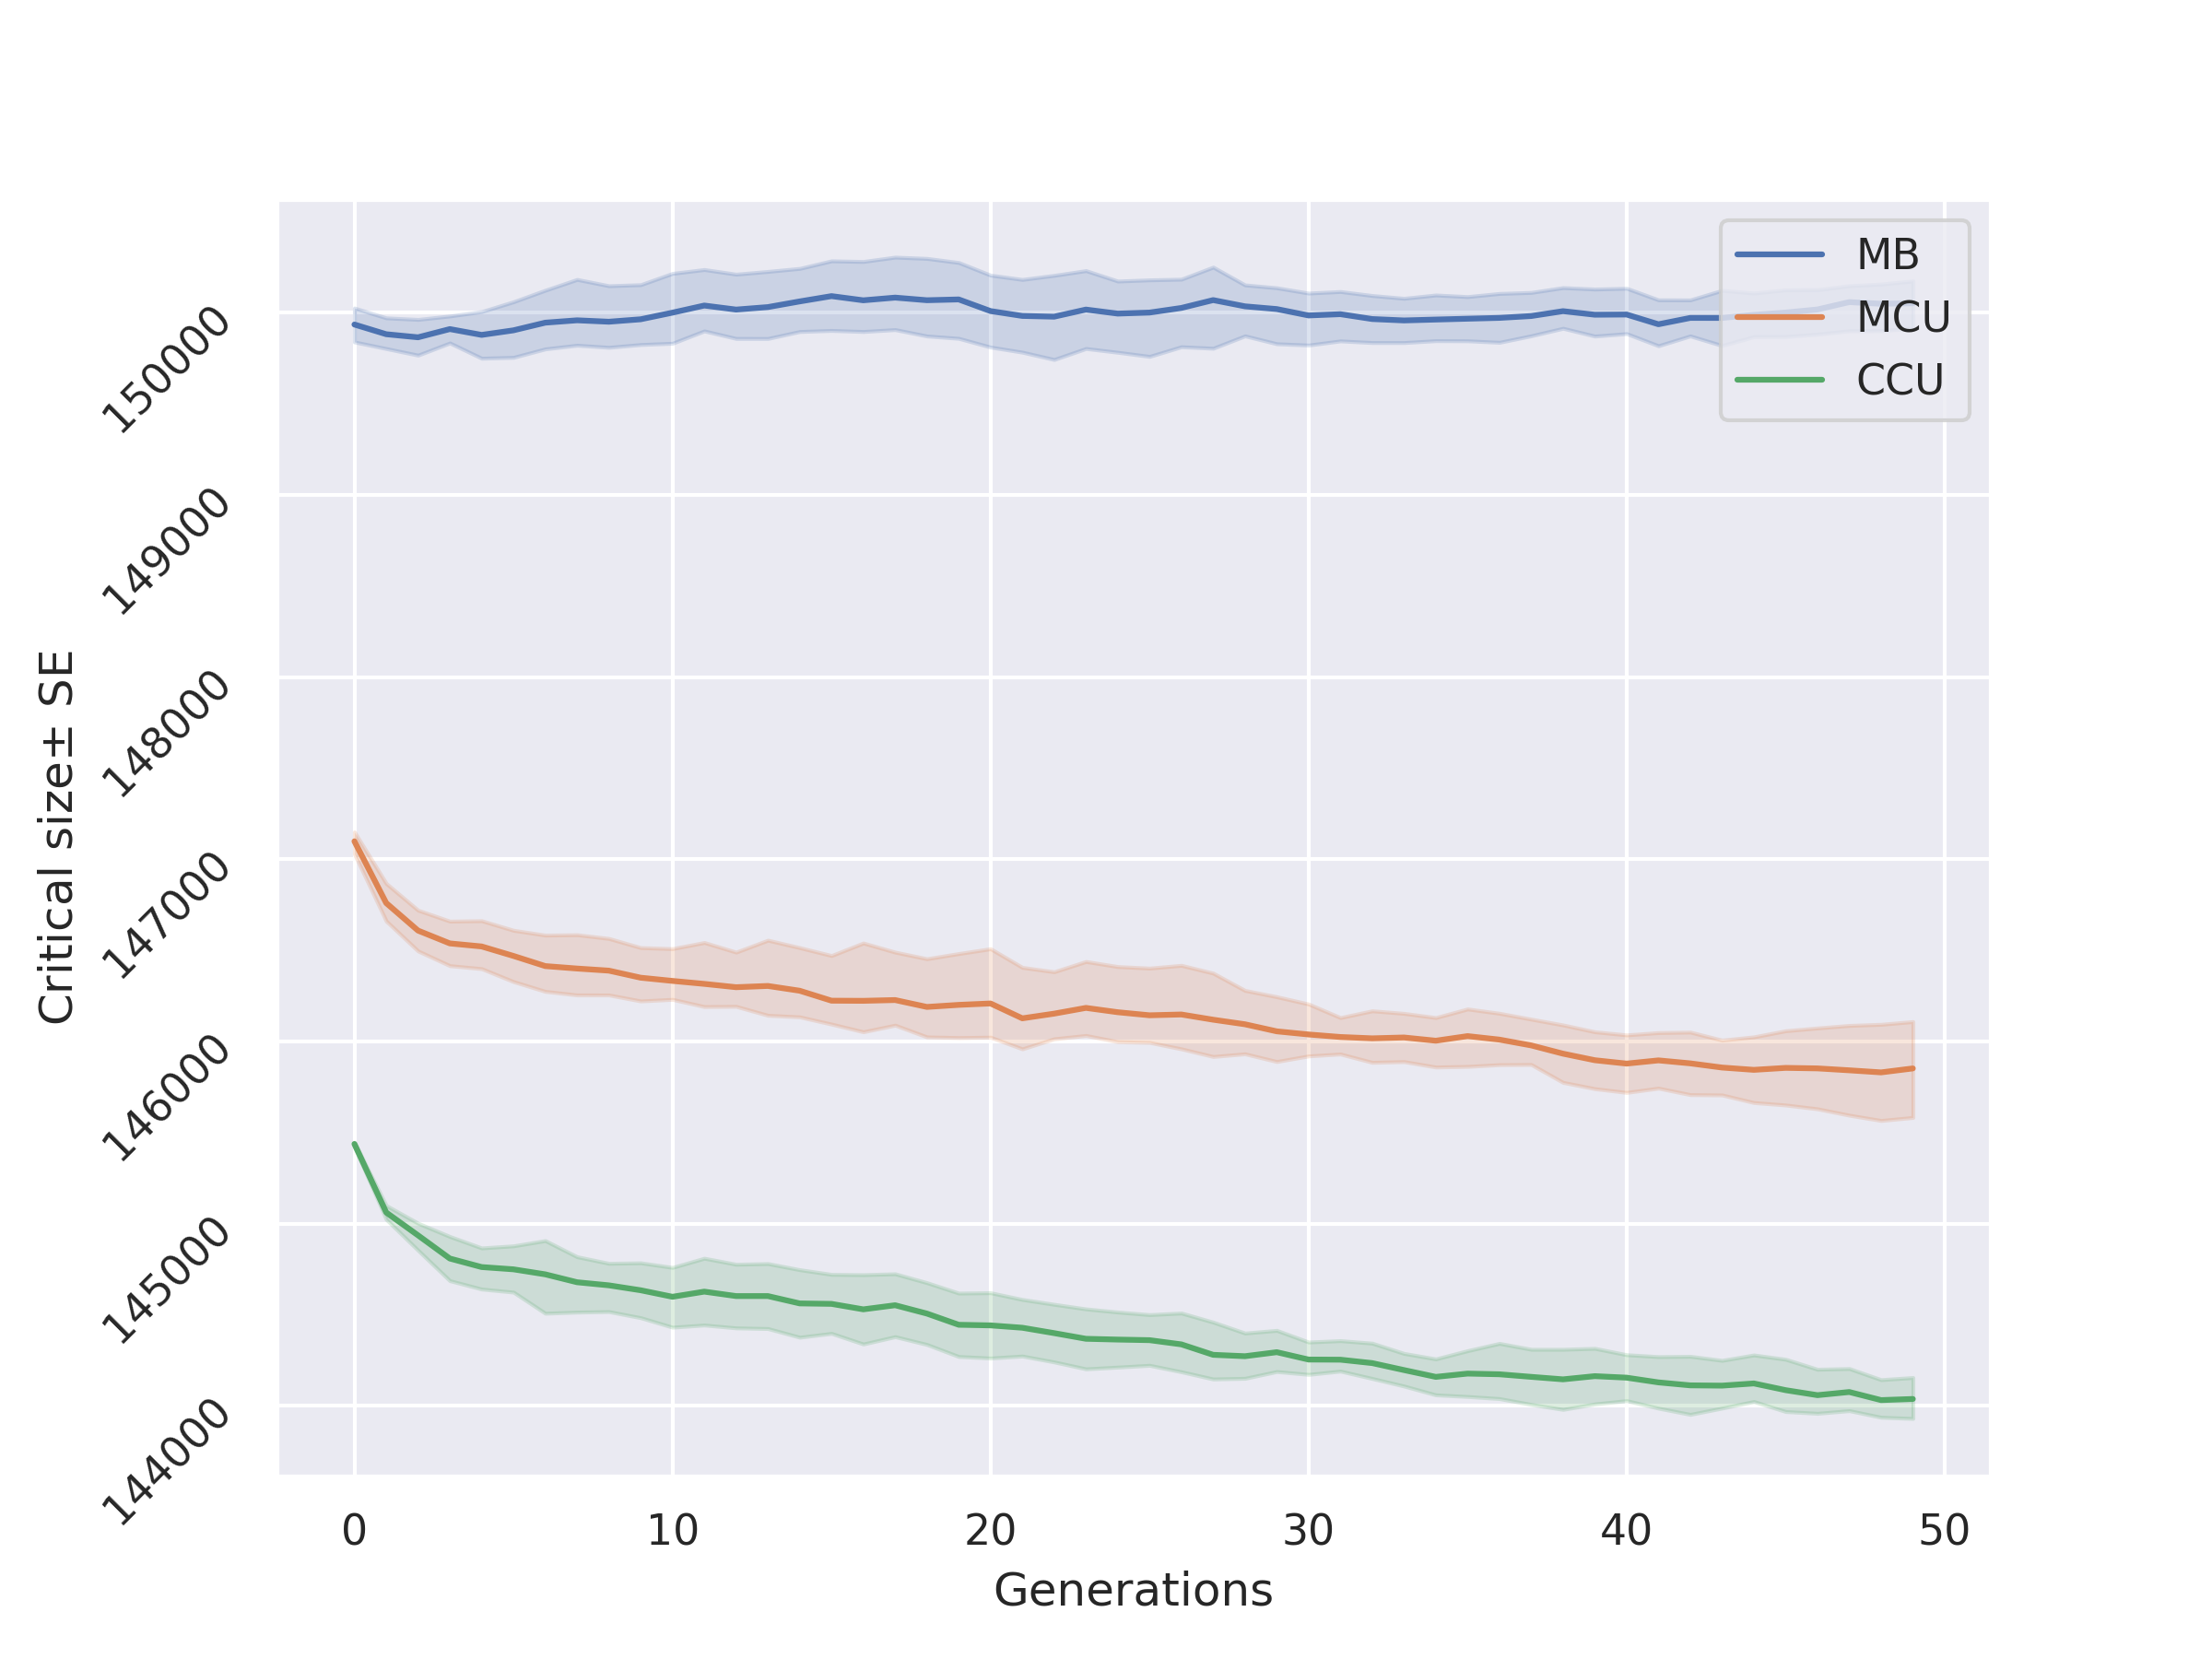
\includegraphics[width=0.9\textwidth]{C4/Figs/mc}
  \caption{Timeseries for initial critical size}
  \label{mc}
  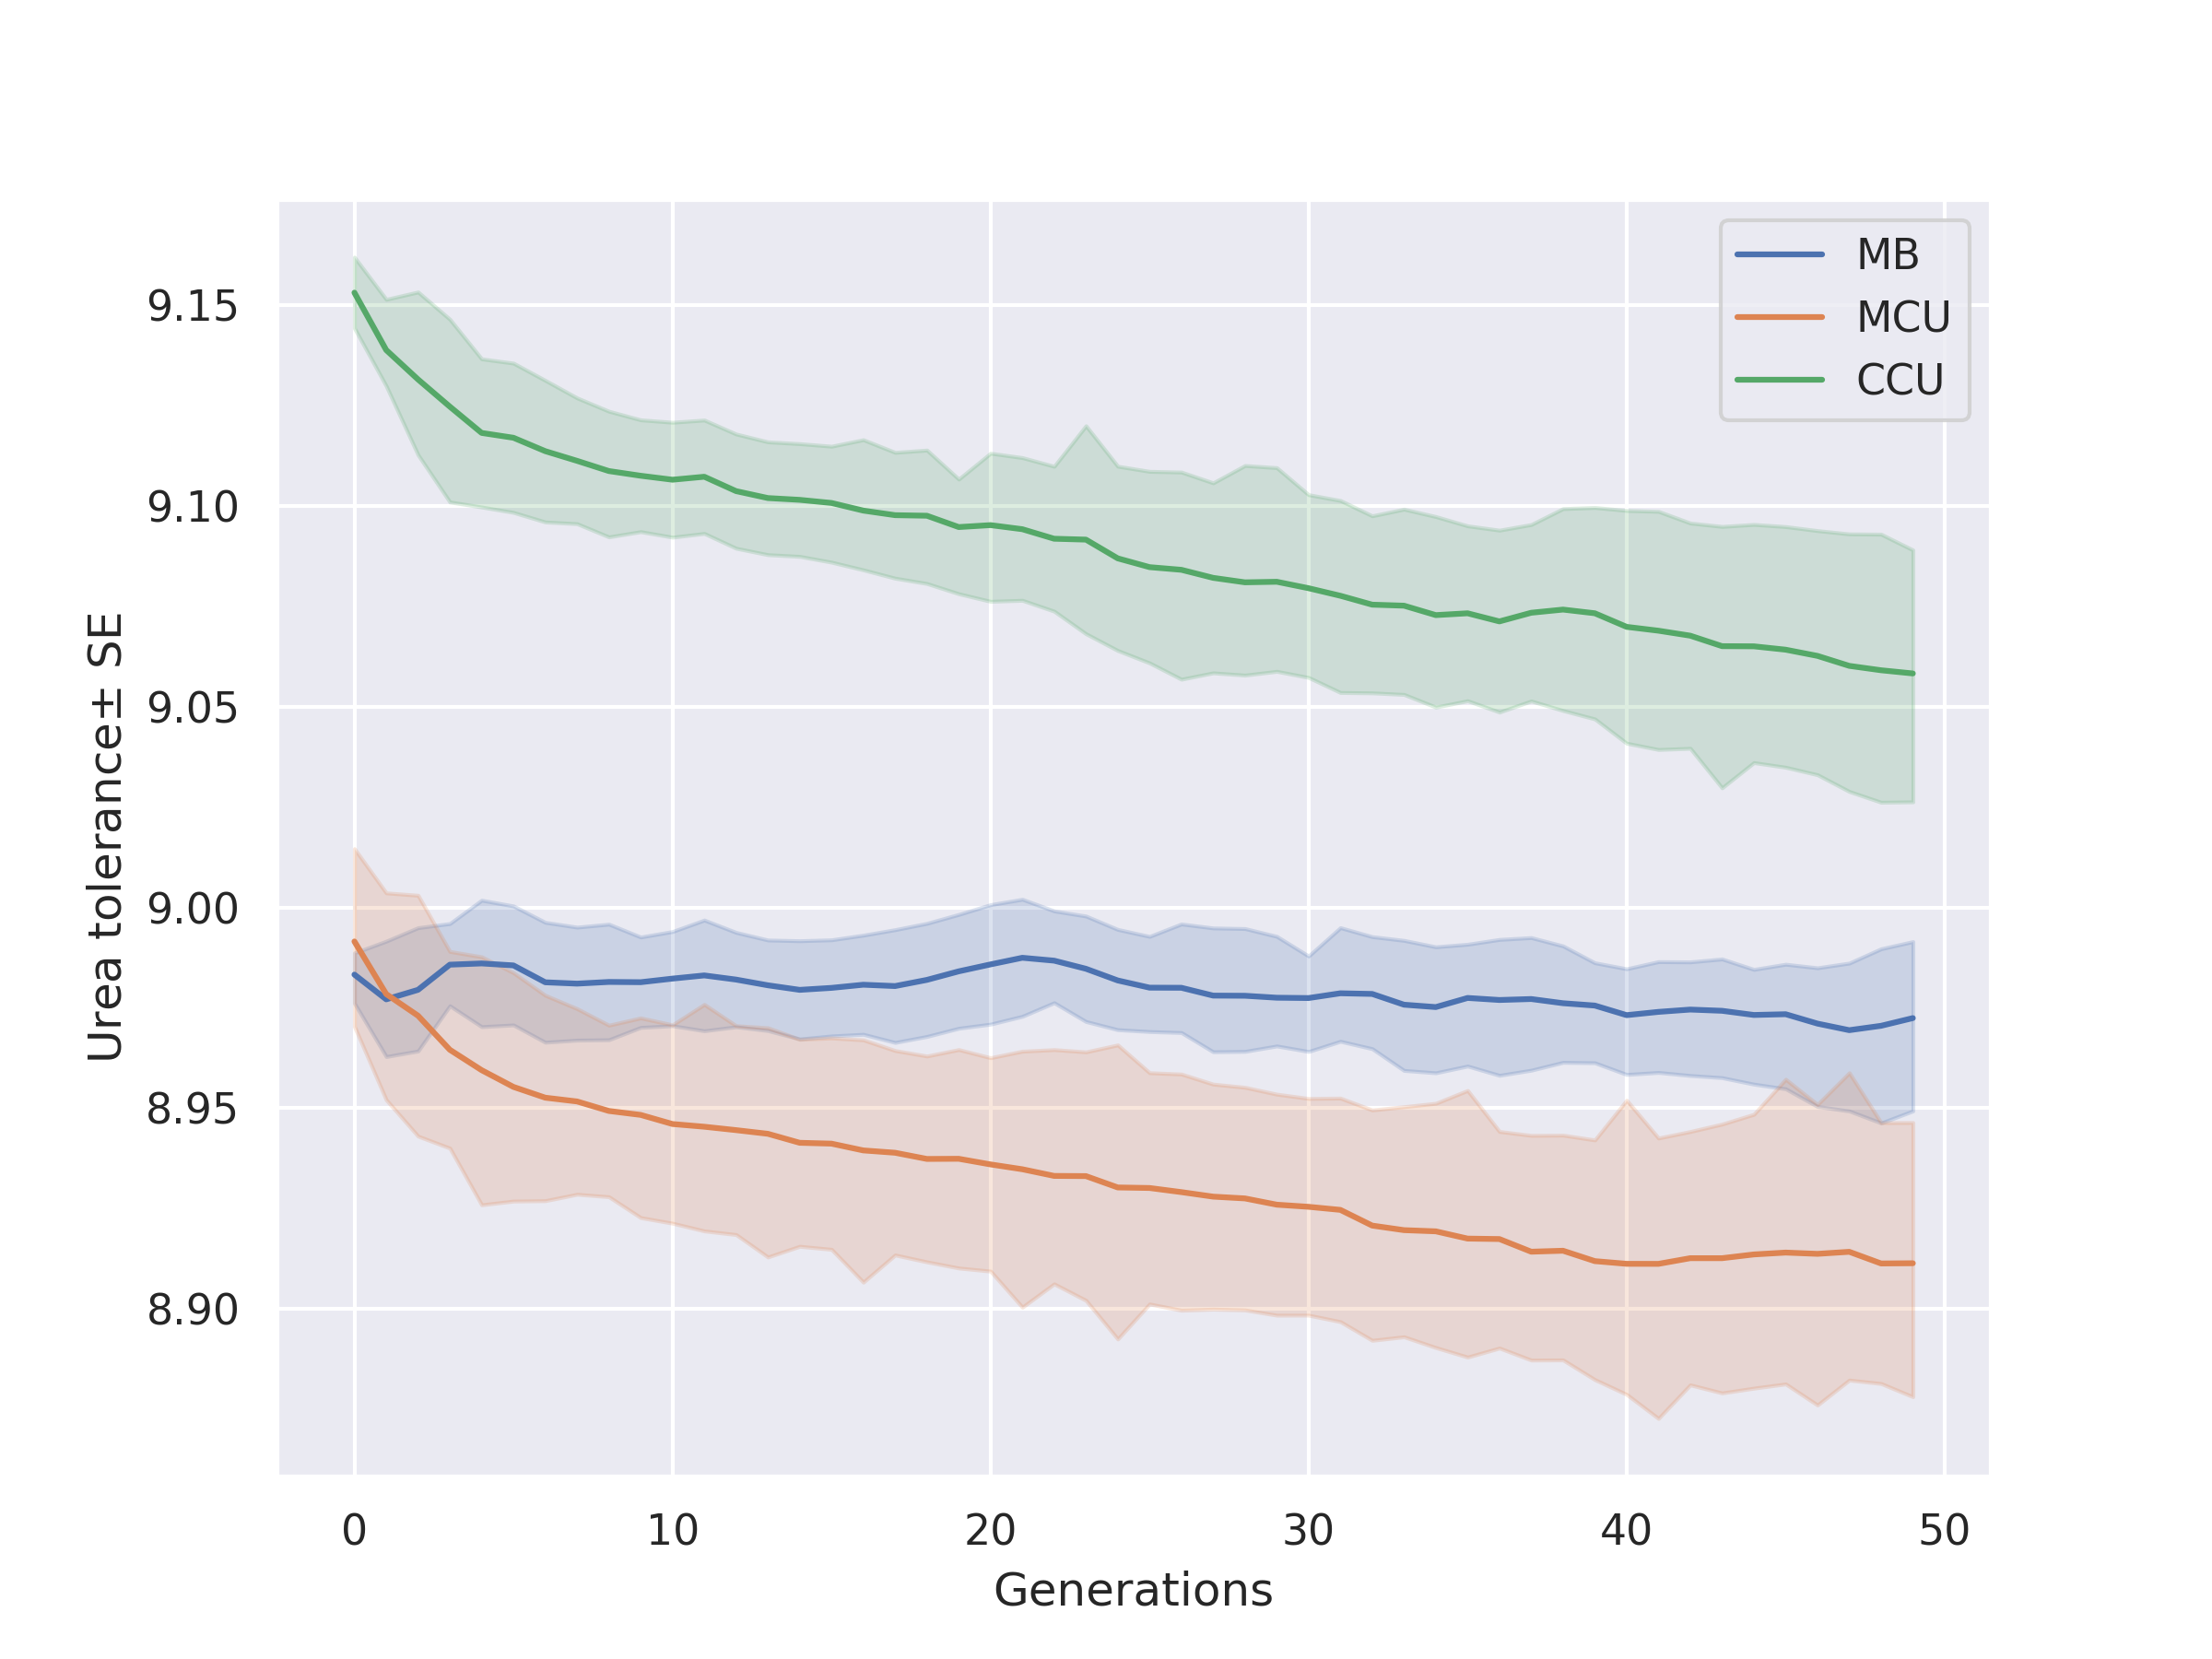
\includegraphics[width=0.9\textwidth]{C4/Figs/wtol}
  \caption{Timeseries for initial waste tolerance}
  \label{wtol}
\end{figure}
\newpage
\section{Effects of Variation on the Evolution of Larval Trait Parameters}
The source of variation in the model comes from the initial variation in the larval trait parameters, given as certain standard deviation in the respective initial distribution as well as from the heritibility of the mid-parent value during the inheritance of the larval trait parameters. The simulations show how these sources of variations play an important role in determining the evolutionary routes taken to acheive greater competitive ability by having maximum survivorship.
\subsection{Variation in the Initial Distribution of Larval Trait Parameters}
When timeseries are plotted for the larval trait parameters, the variation in the initial distribution of these trait parameters determine the maxima that can be achieved to increase the fitness. From fig(a), fig(b) and fig(c), it is seen that differences in variation of these trait values, maxima reached are different with similar initial mean trait values. If the initial variation in efficiency is very high compared initial variation in feeding rate, then feeding rate does not reach higher feeding rate after few generations unlike of the timeseries simulations performed with lower initial variation in the efficiency. Depending on the initial variation in each trait separately, traits can evolve differently, since these trait parameters interact with each other to give complex phenotypes suxh as body size, time to rach critical size and survivorship.
\subsection{Heritibility in Mid-parent Value}

%\section{Discussion}

\pagebreak
%\renewcommand\bibname{{References}}
\bibliography{References}
\bibliographystyle{plain}
